% This document is made freely avaiable through the CC0 1.0 Universal license (logo excluded).
% Similar material avaiable at https://github.com/noahhaworth/CAD_Material
% Things to fix:
%		make wording more accurate + spelling check
%		considering adding color
%		missing diameter for die problem
%		make sure to include UFO equations
%		recheck image resolutions, maybe decrease for file size
%		ensure all figures are well defined

\documentclass{article}
\usepackage[utf8]{inputenc}
\usepackage[legalpaper, landscape,top=.5in,right=1.5in,left=1.5in,bottom=1.5in]{geometry}
\usepackage{ragged2e}
\usepackage{graphicx}
\usepackage{float}
\usepackage{setspace}
\usepackage[labelfont=bf]{caption}
\usepackage{hyperref}
\usepackage{array}
\usepackage{xcolor}
\hypersetup{colorlinks=true, urlcolor=blue}

\begin{document}
\definecolor{noah}{HTML}{ffffff}
\pagecolor{noah}
\center
\Huge{\textbf{SolidWorks Parts Practice Problems}\\[3mm] \hrule
\vspace{4mm}
\includegraphics[width=0.15\textwidth]{~/Documents/github/nwh.png}\\[4mm] 
\justify\normalsize
\textbf{Information:} The following problems were originally part of a three hour SolidWorks part exam. You are free to do as you please with this document. More material similar to this can be found \href{https://github.com/noahhaworth/CAD_Material}{here}.\\[10mm]
\newpage
\newgeometry{top=.5in,right=1.5in,left=1.5in,bottom=1.5in}

%problem 1
\textbf{P1}
\begin{figure}[H]
  \centering
  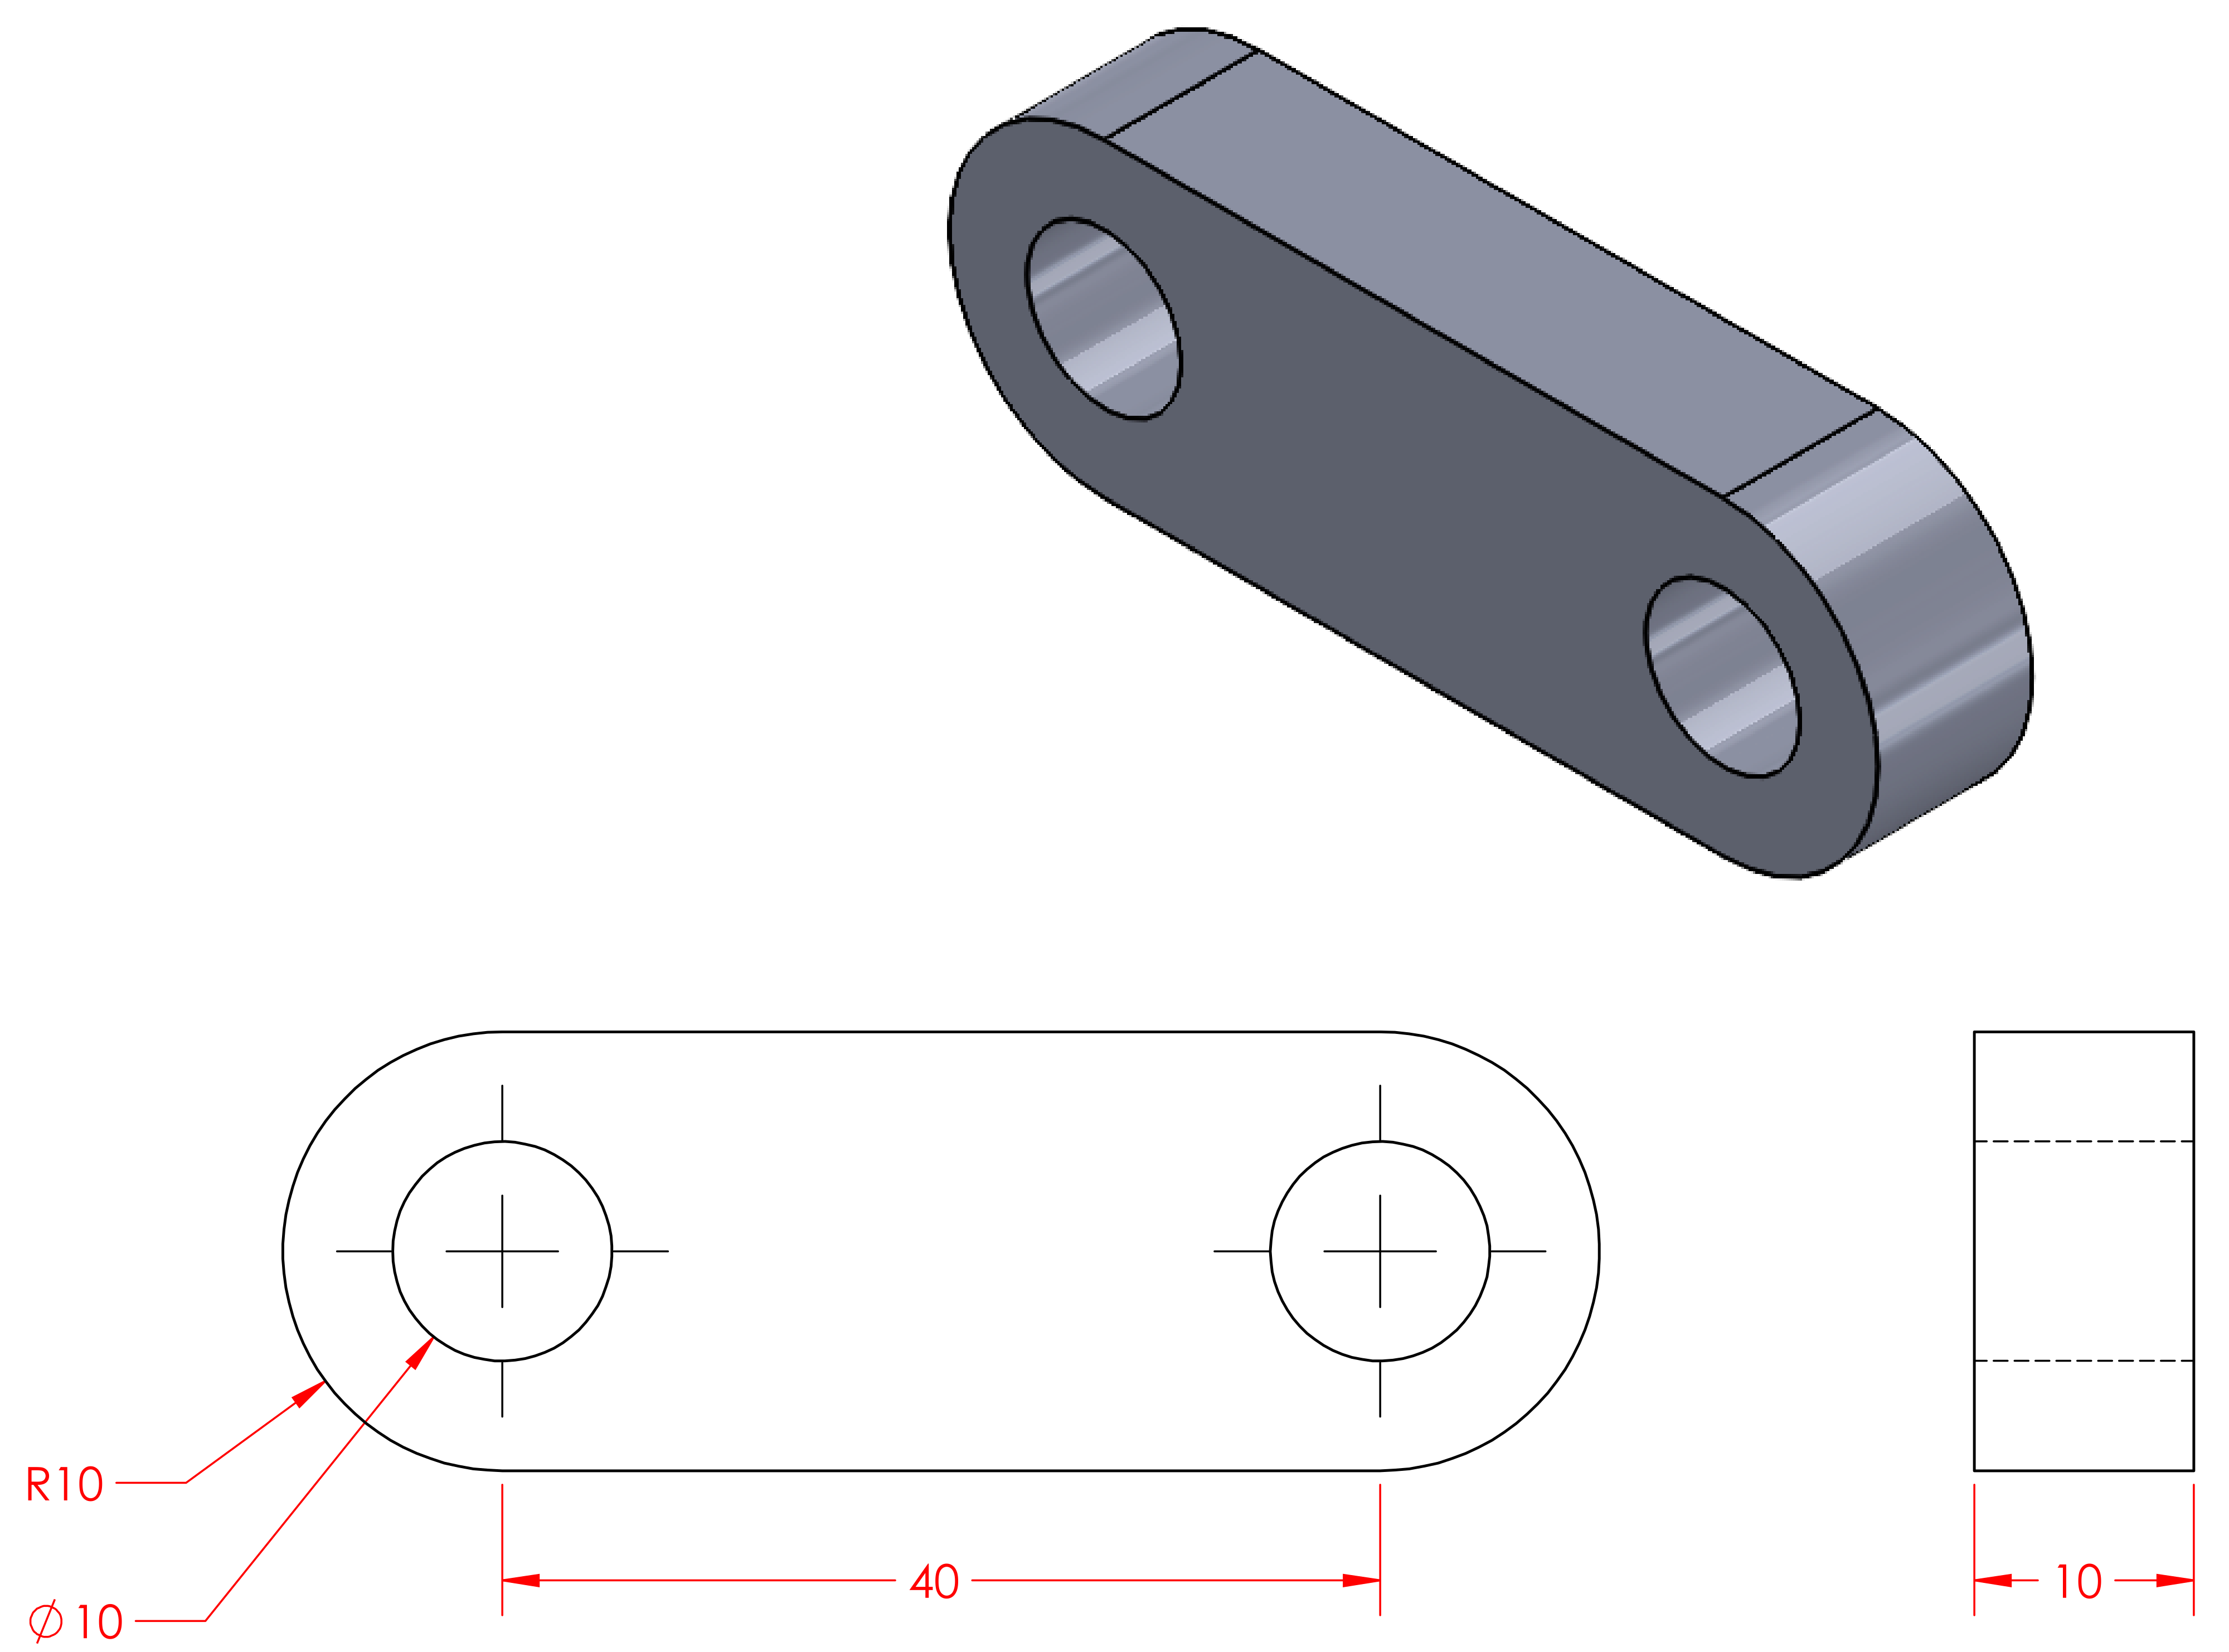
\includegraphics[width=.68\linewidth]{images/1.png}  
  \caption{Link}
  \label{fig:1}
\end{figure}
\noindent Please create the 3D body seen above in \textit{Figure 1} using SolidWorks.

%problem 2
\textbf{P2}
\begin{figure}[H]
  \centering
  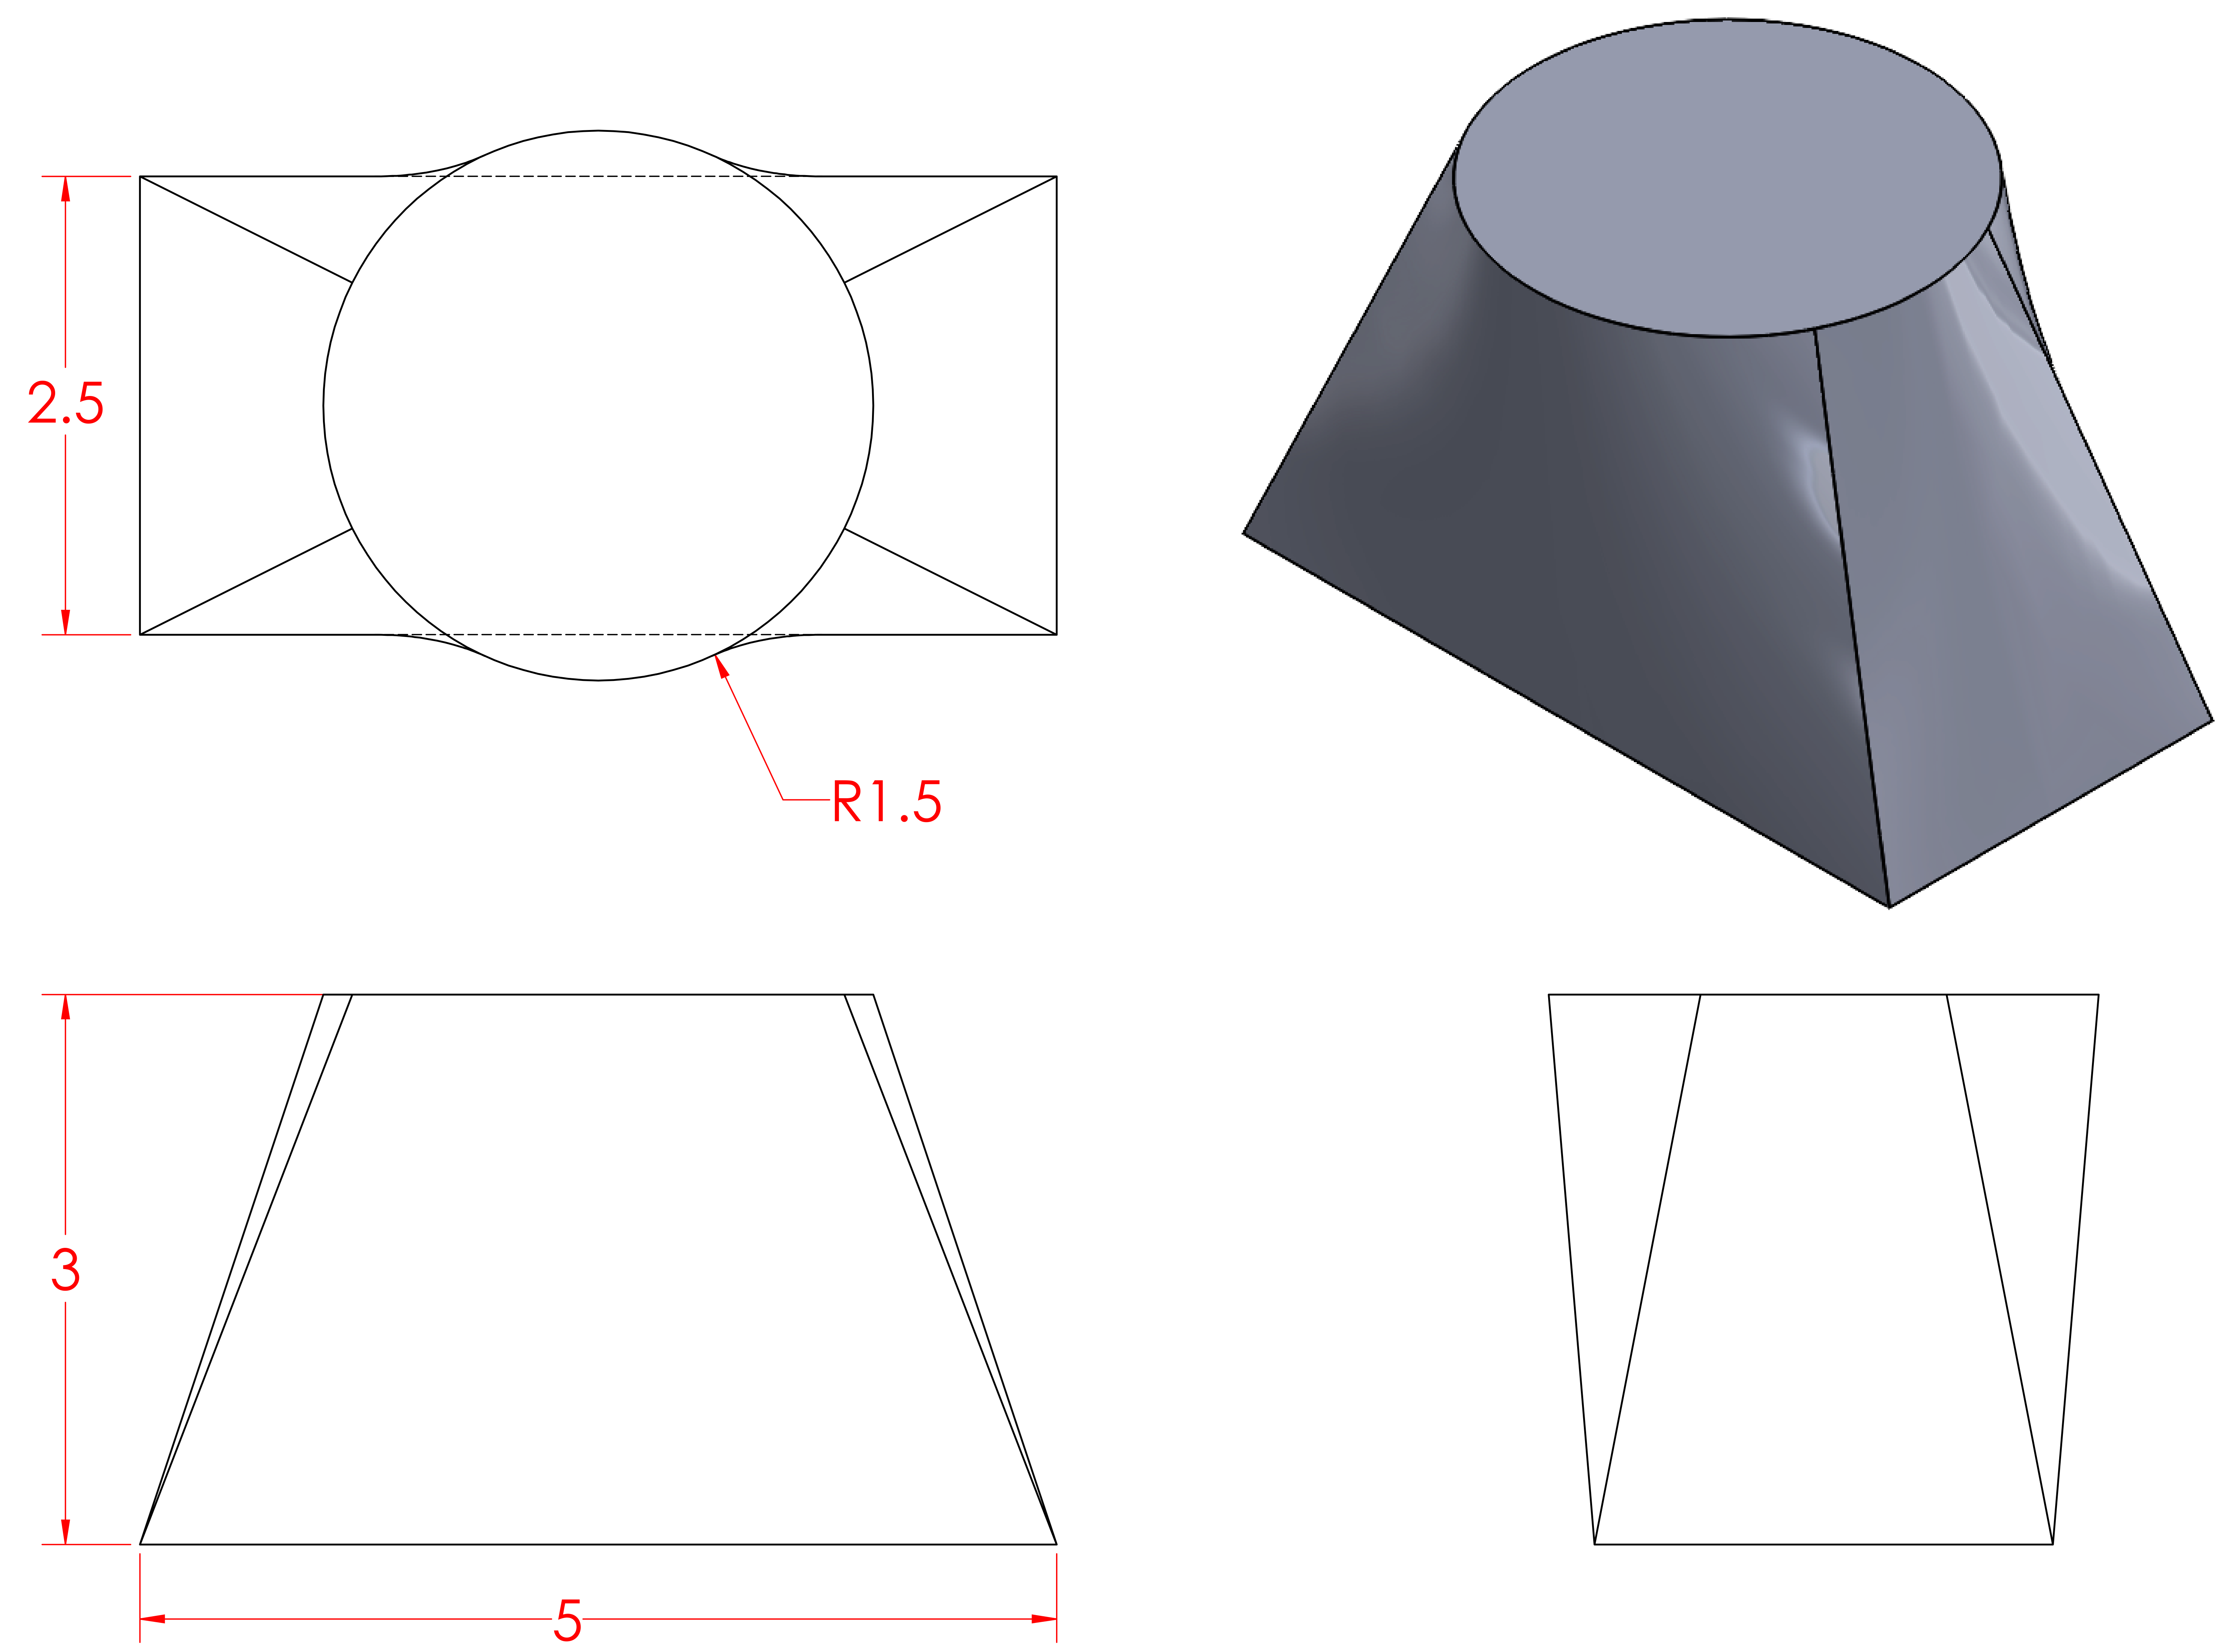
\includegraphics[width=.68\linewidth]{images/2.png}  
  \caption{Rectangle to Circle}
  \label{fig:2}
\end{figure}
\noindent Please create the 3D body seen above in \textit{Figure 2} using SolidWorks.

%problem 3
\textbf{P3}
\begin{figure}[H]
  \centering
  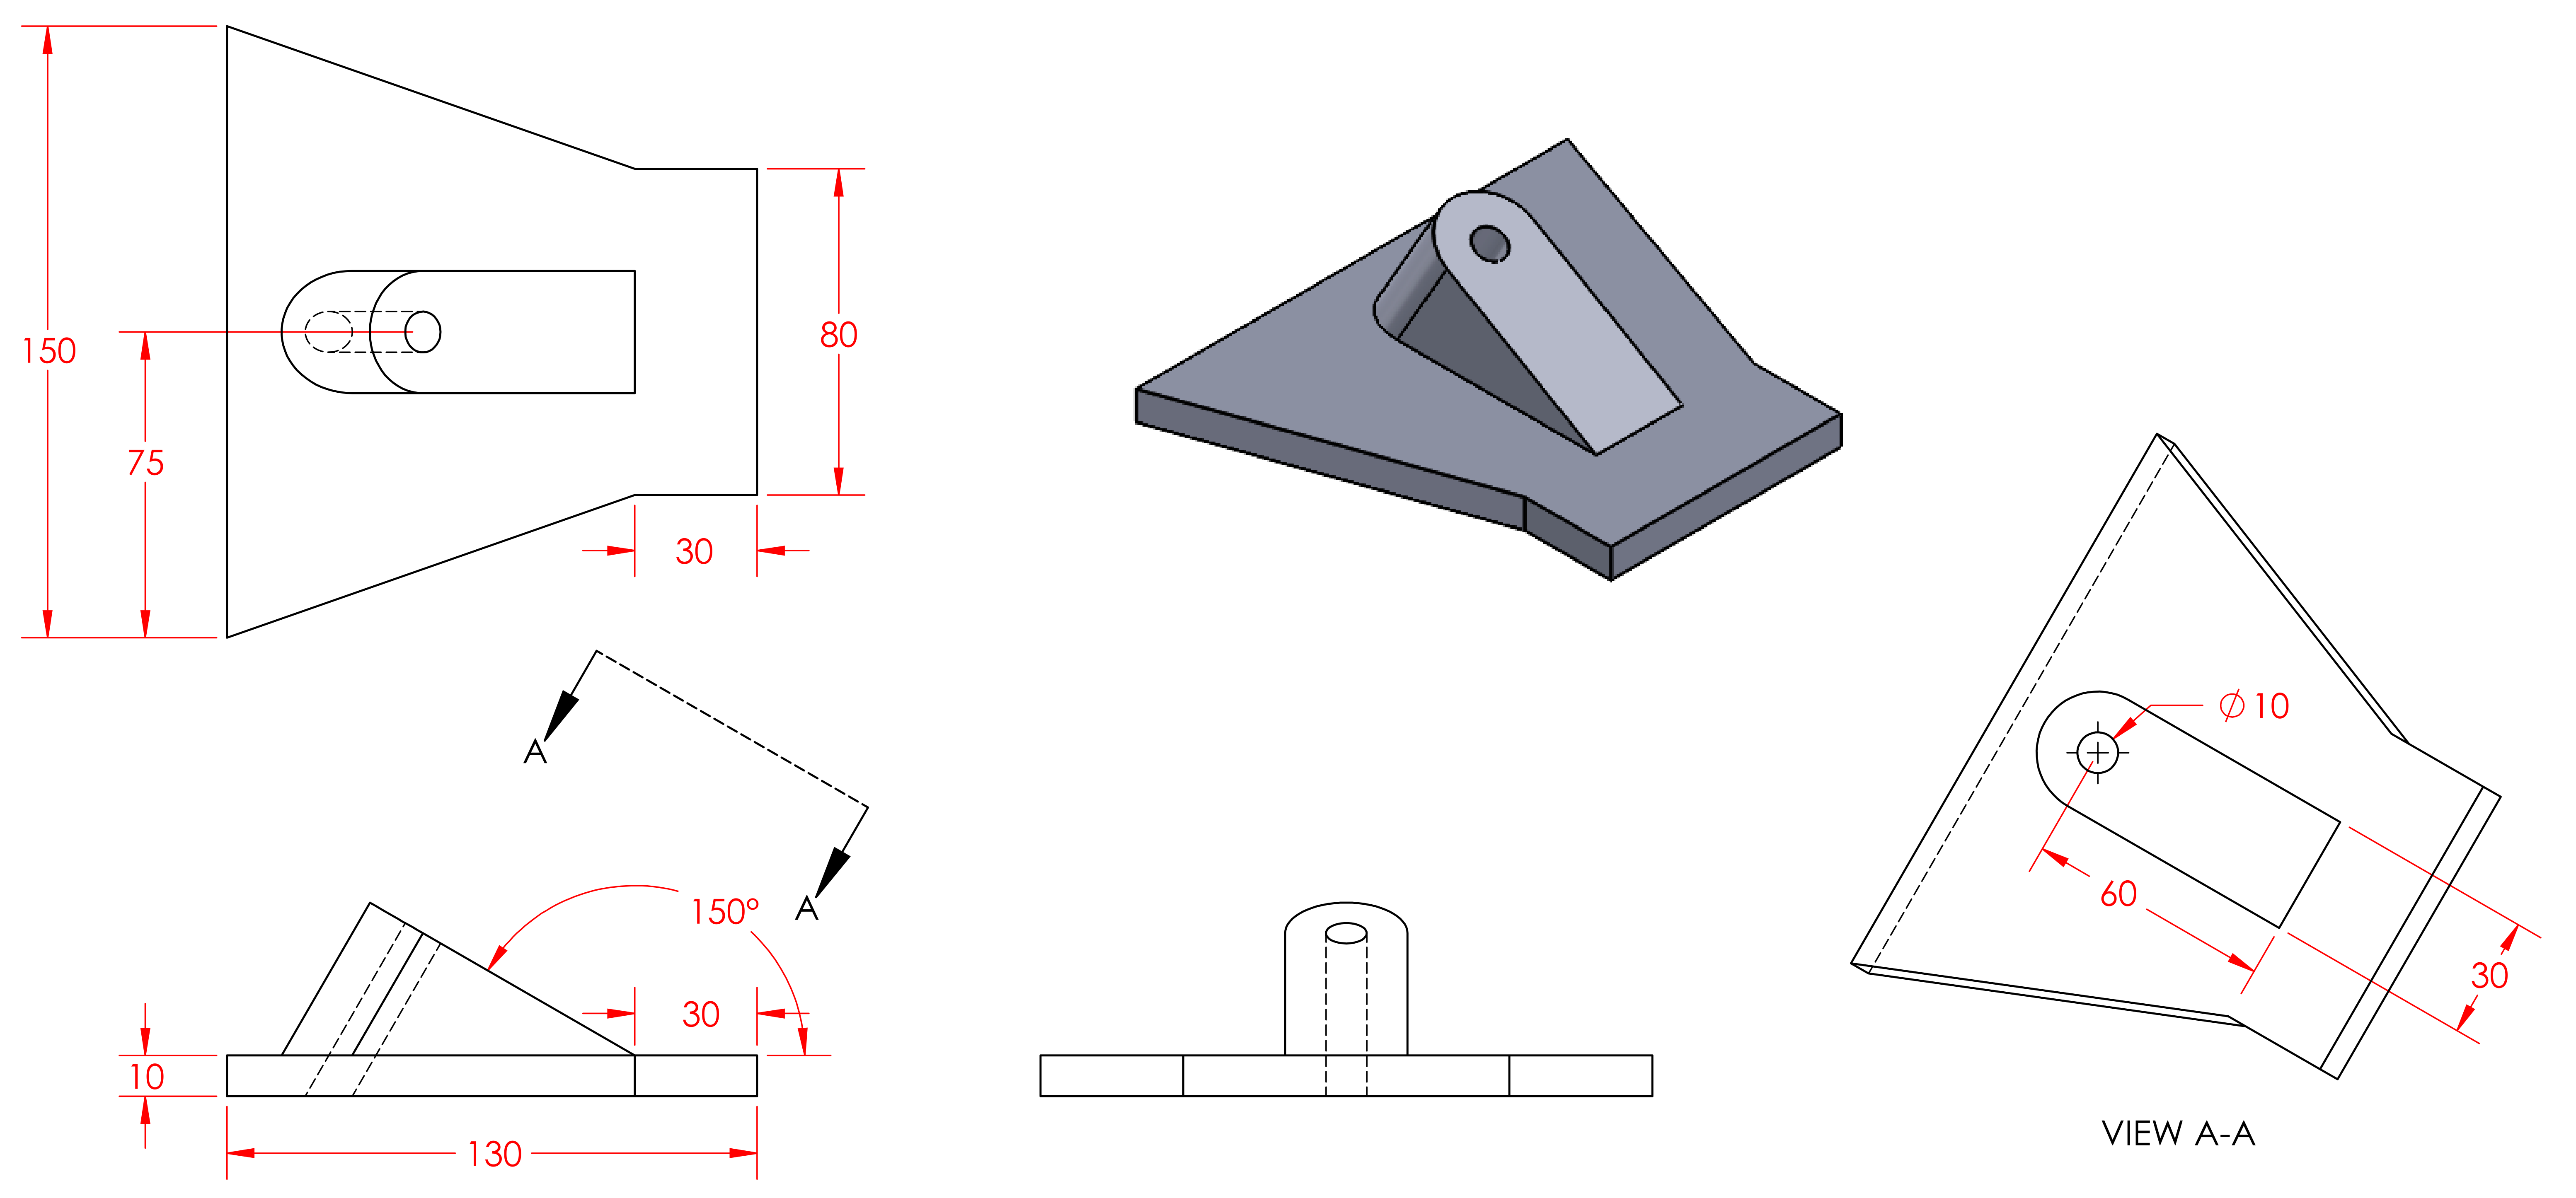
\includegraphics[width=1.075\linewidth]{images/3.png}  
  \caption{Incline}
  \label{fig:3}
\end{figure}
\noindent Please create the 3D body seen above in \textit{Figure 3} using SolidWorks.

%problem 4
\textbf{P4}
\begin{figure}[H]
  \centering
  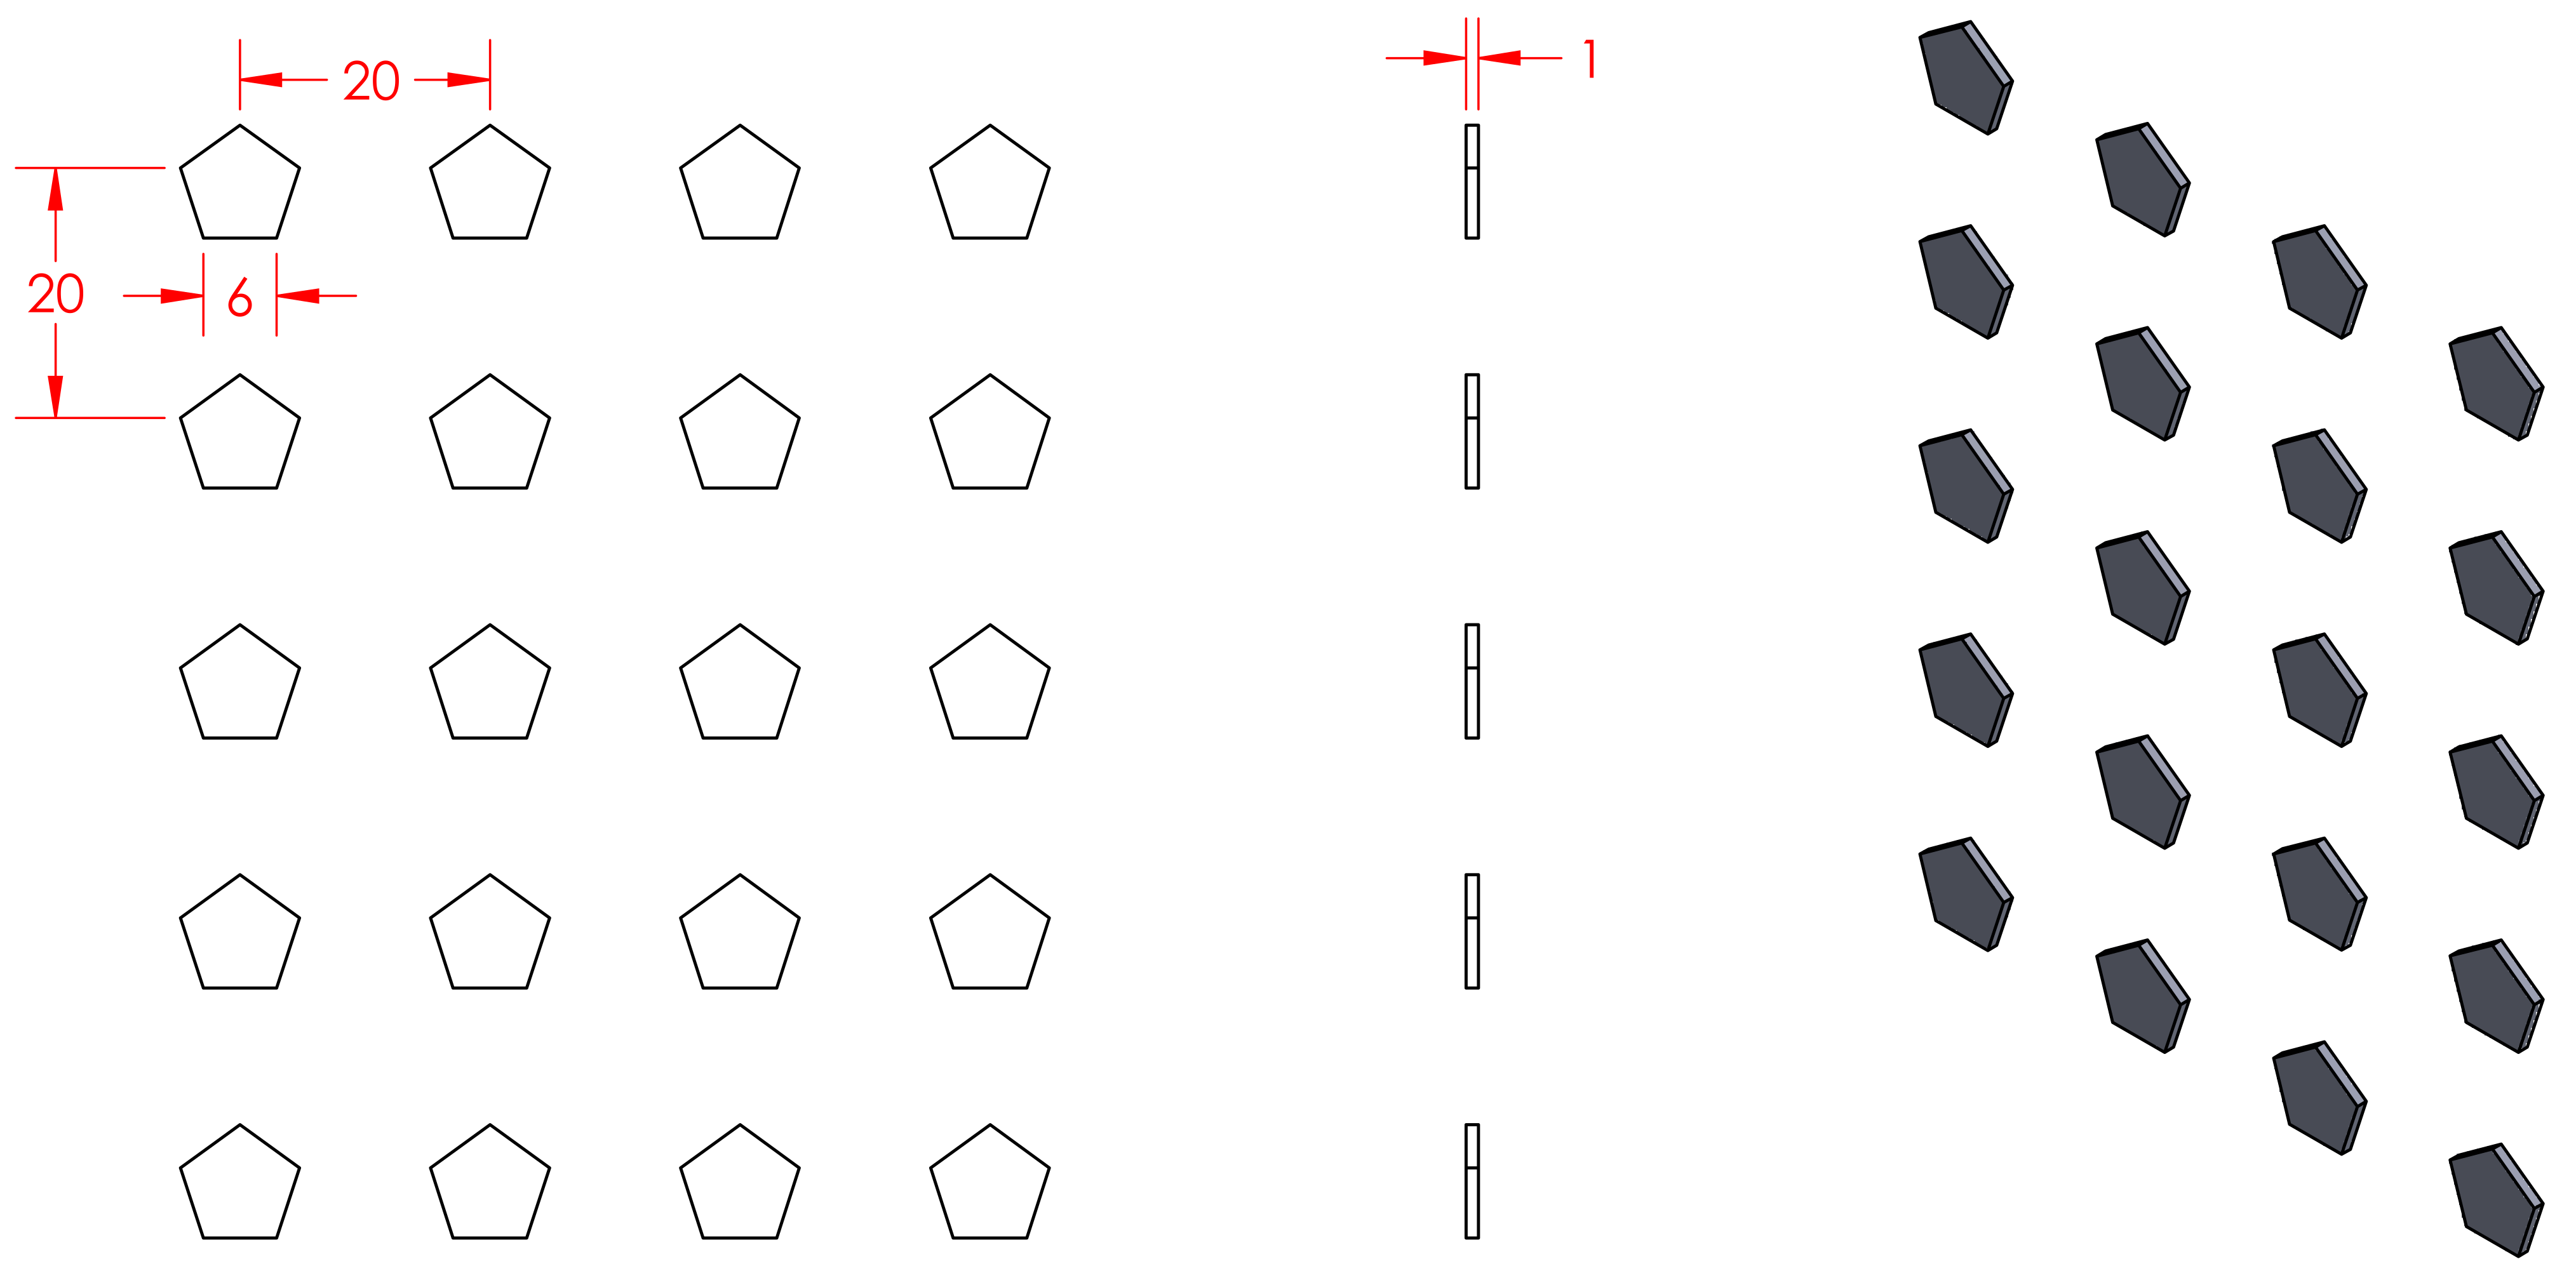
\includegraphics[width=\linewidth]{images/4.png}  
  \caption{Pentagons}
  \label{fig:4}
\end{figure}
\noindent Please create the 3D body seen above in \textit{Figure 4} using SolidWorks.

%problem 5
\textbf{P5}
\begin{figure}[H]
  \centering
  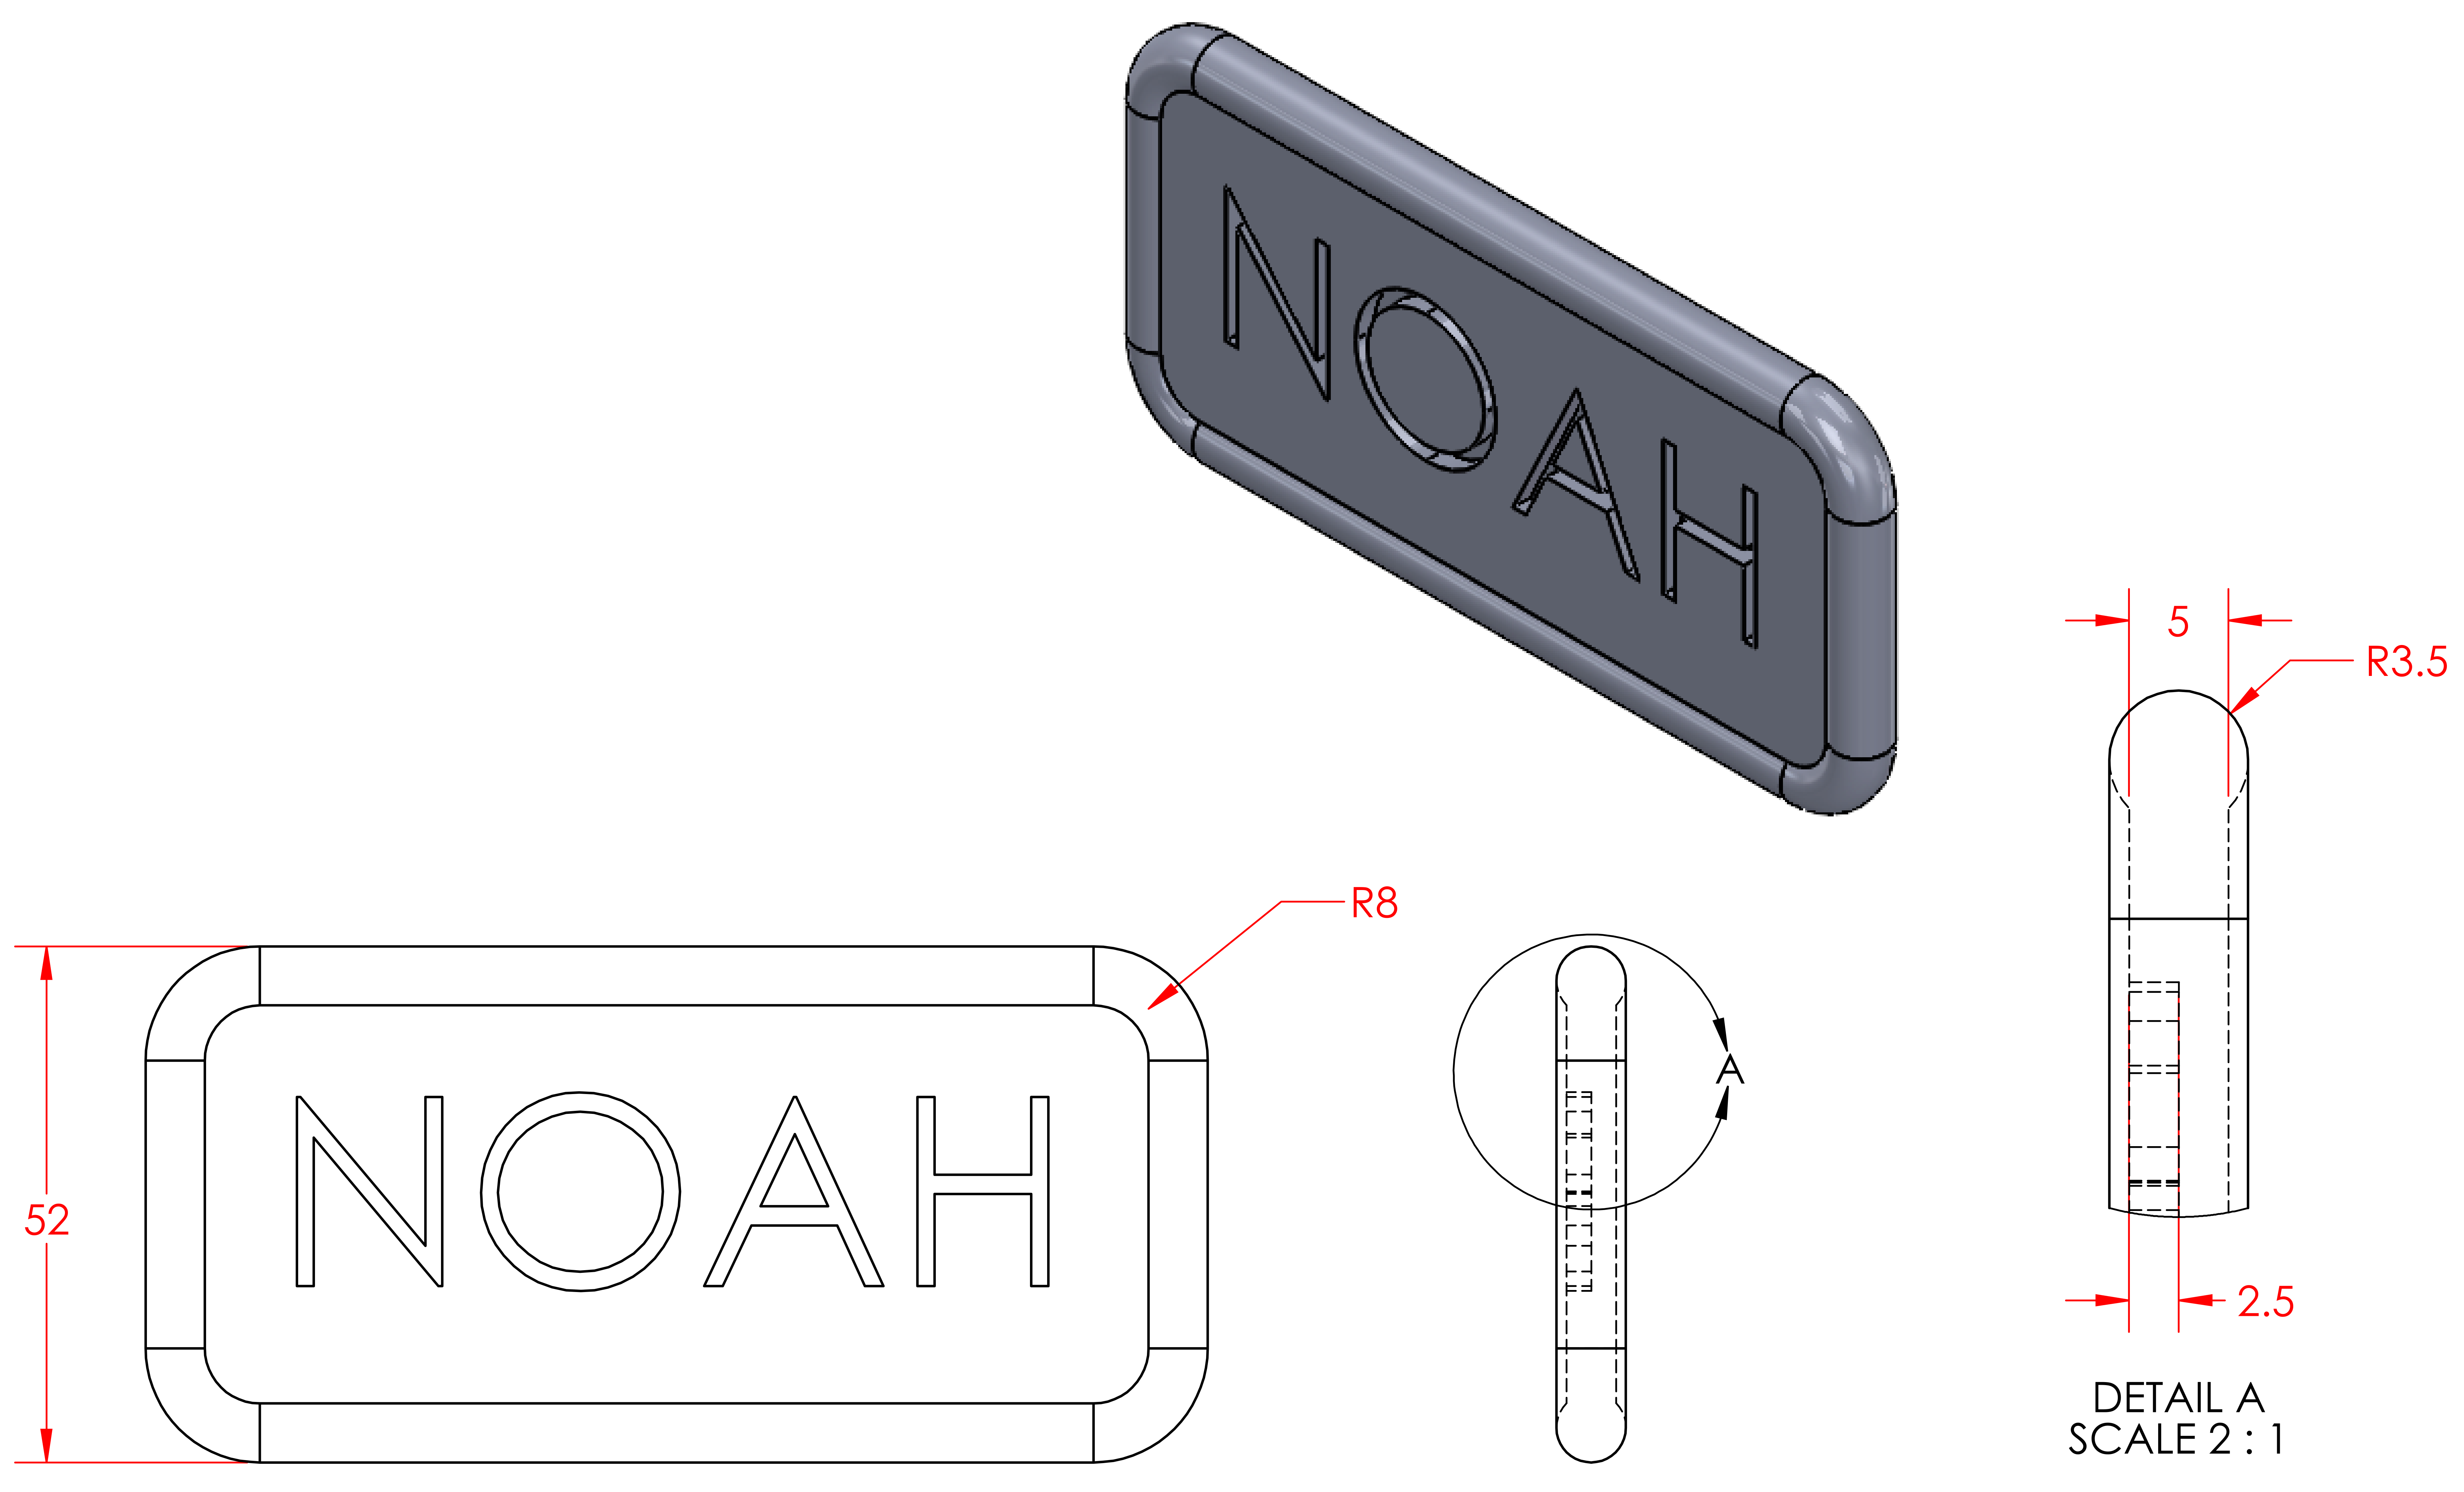
\includegraphics[width=.825\linewidth]{images/5.png}  
  \caption{Name Tag}
  \label{fig:5}
\end{figure}
\noindent Please create the 3D body seen above in \textit{Figure 5} using SolidWorks.

%problem 6
\textbf{P6}
\begin{figure}[H]
  \centering
  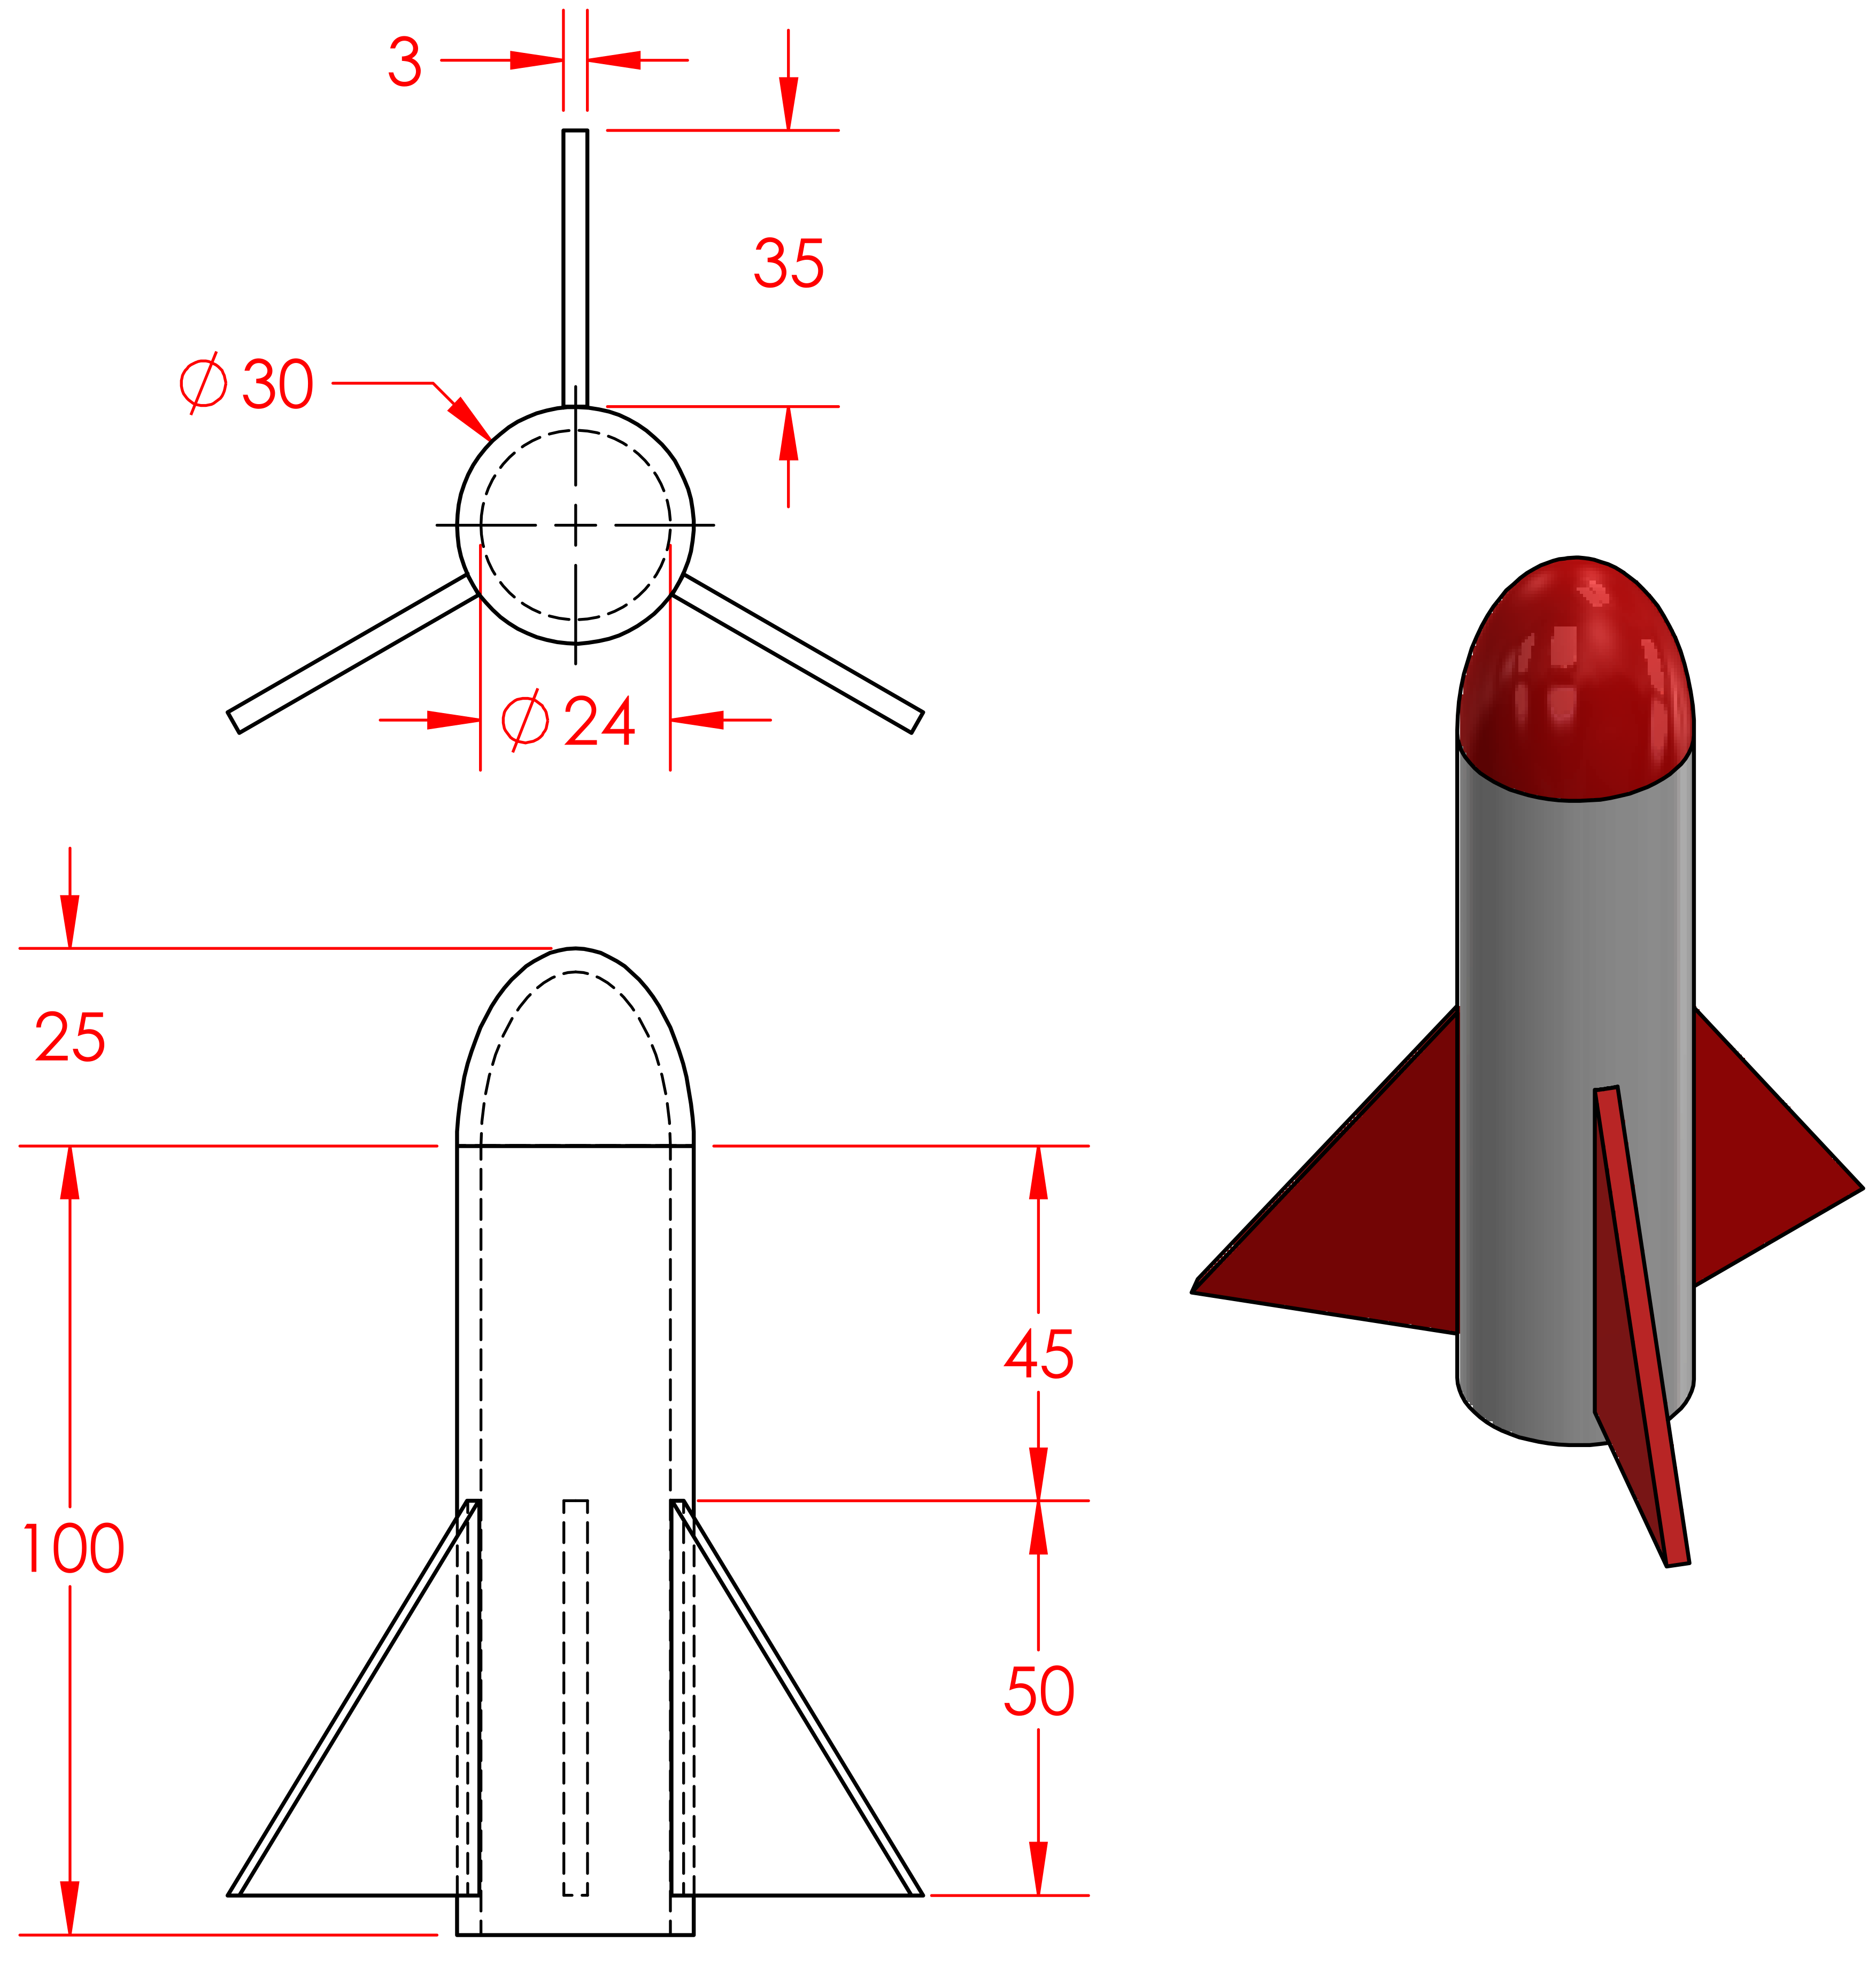
\includegraphics[width=.475\linewidth]{images/6.png}  
  \caption{Robot}
  \label{fig:6}
\end{figure}
\noindent Please create the 3D body seen above in \textit{Figure 6} using SolidWorks.

%problem 7
\textbf{P7}
\begin{figure}[H]
  \centering
  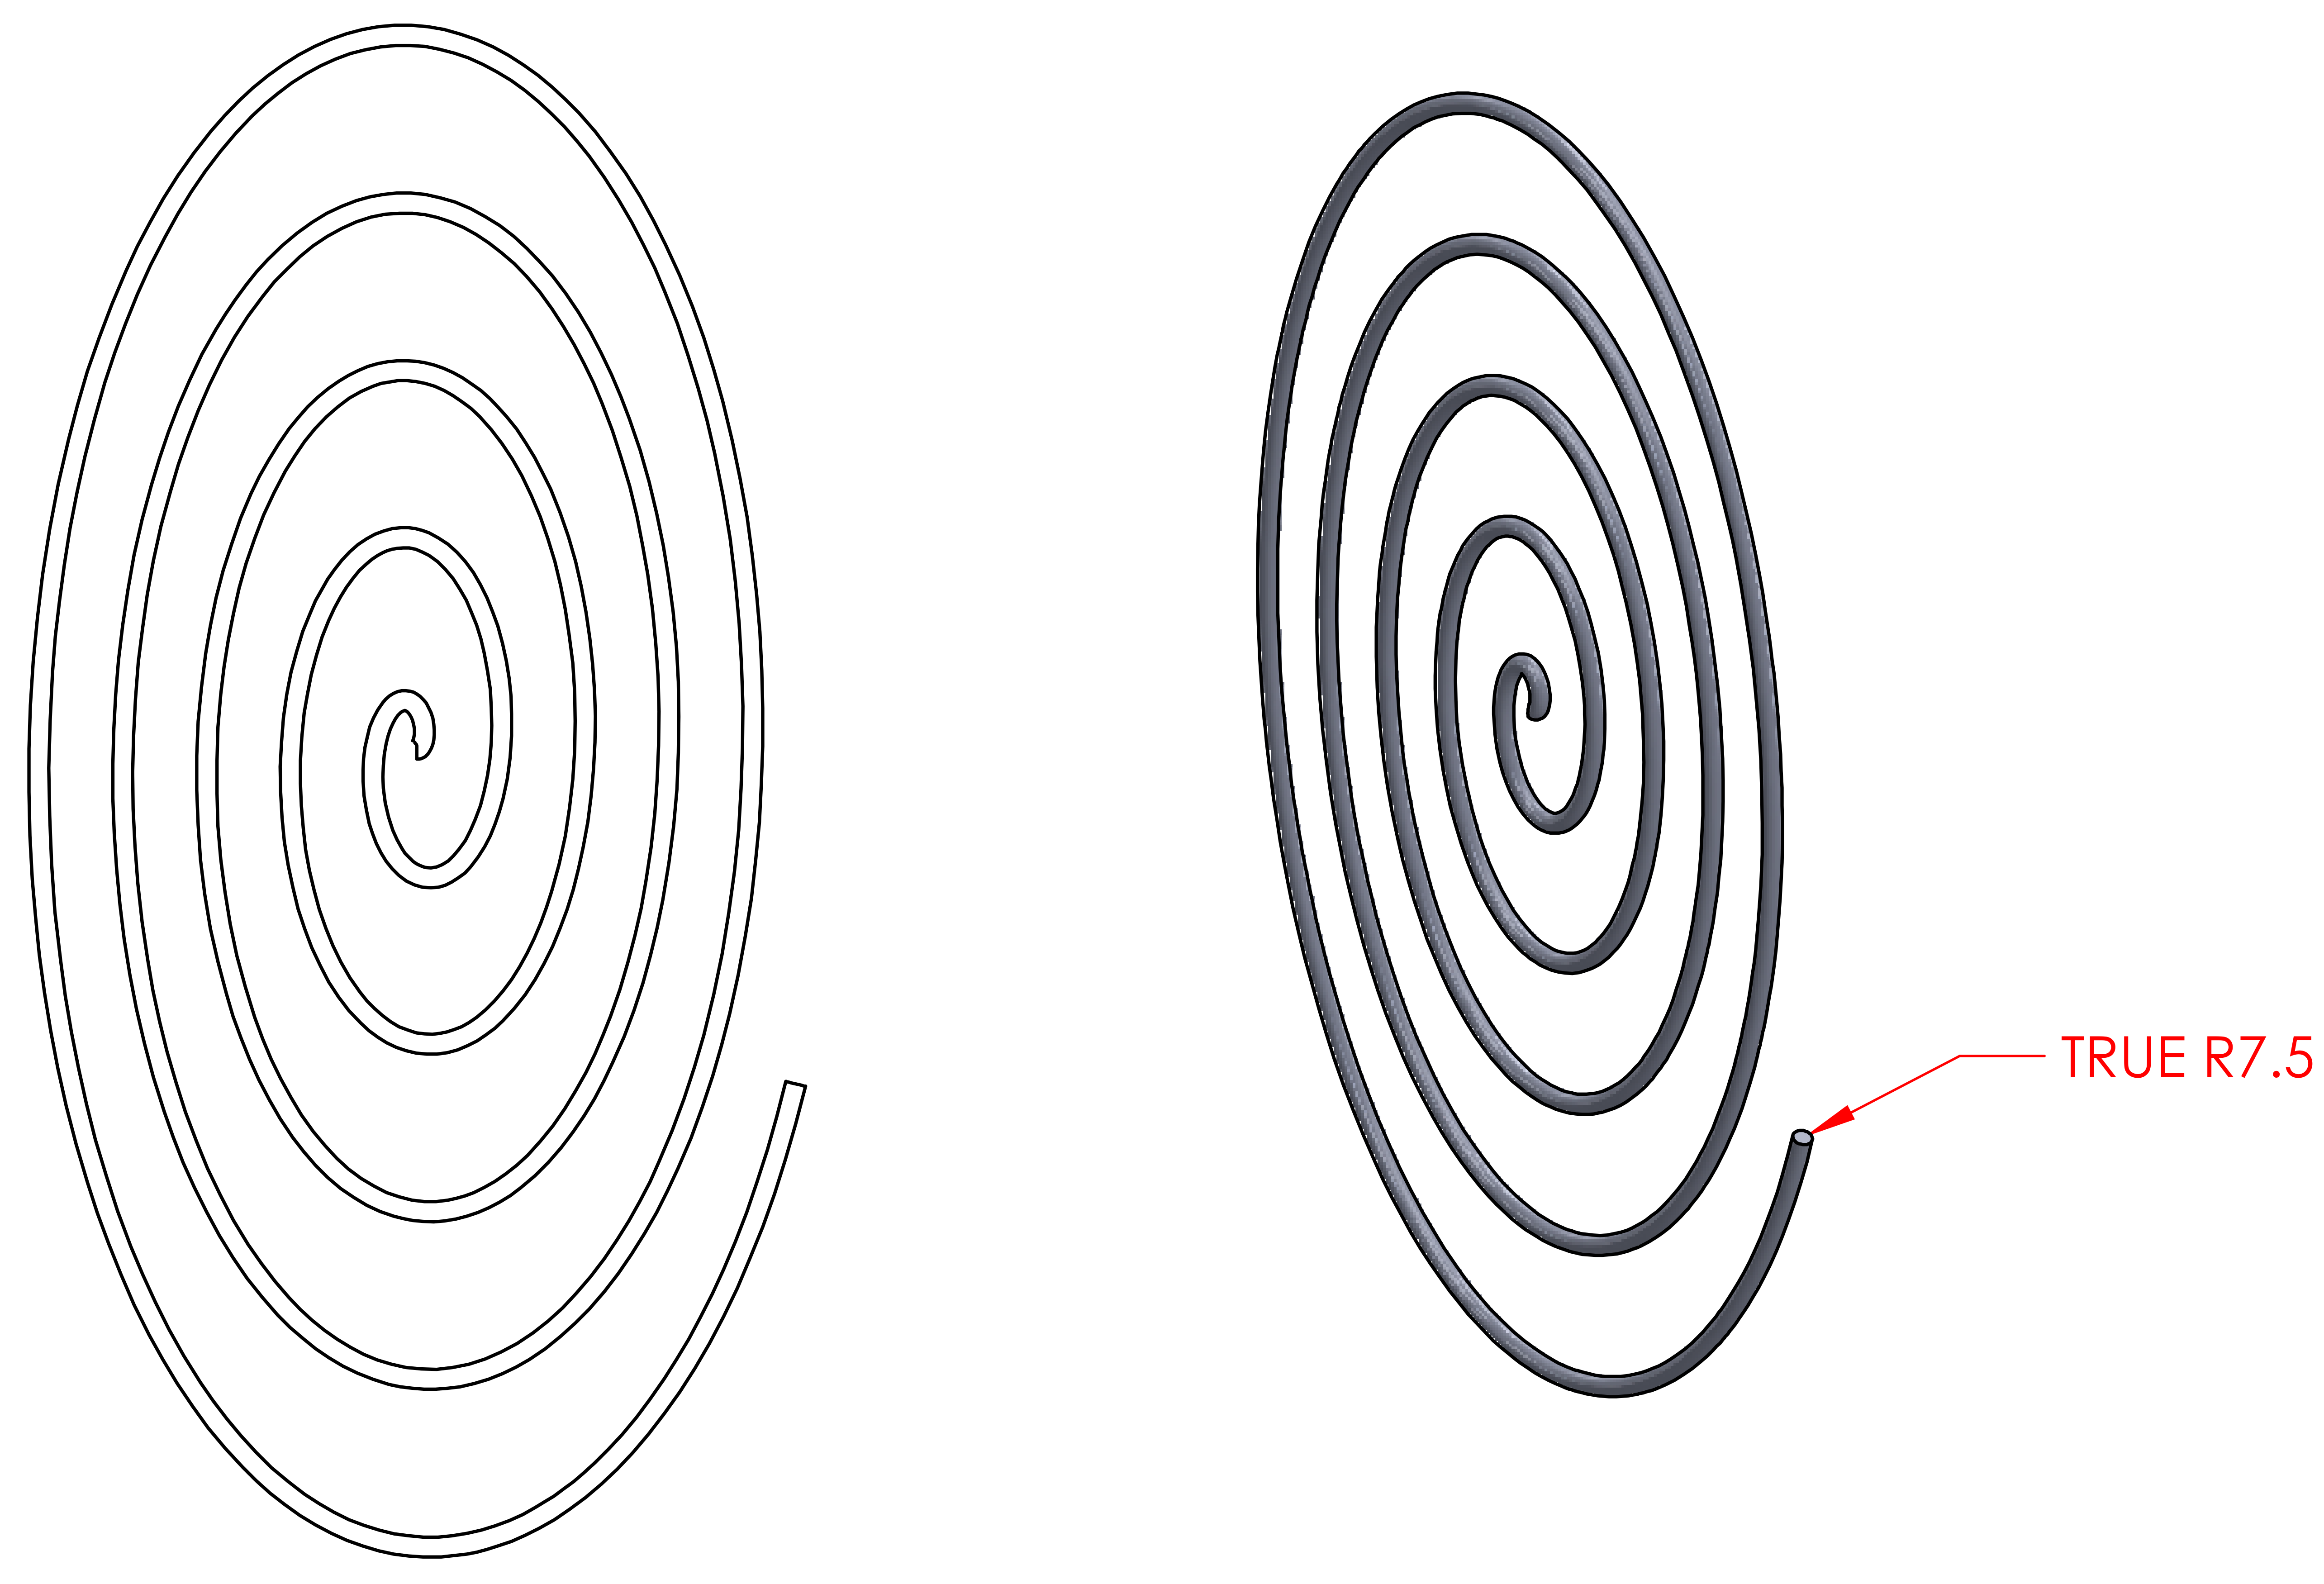
\includegraphics[width=.725\linewidth]{images/7.png}  
  \caption{Fingerprintish}
  \label{fig:7}
\end{figure}
\noindent Please create the 3D body seen above in \textit{Figure 7} using SolidWorks.

%problem 8
\textbf{P8}
\begin{figure}[H]
  \centering
  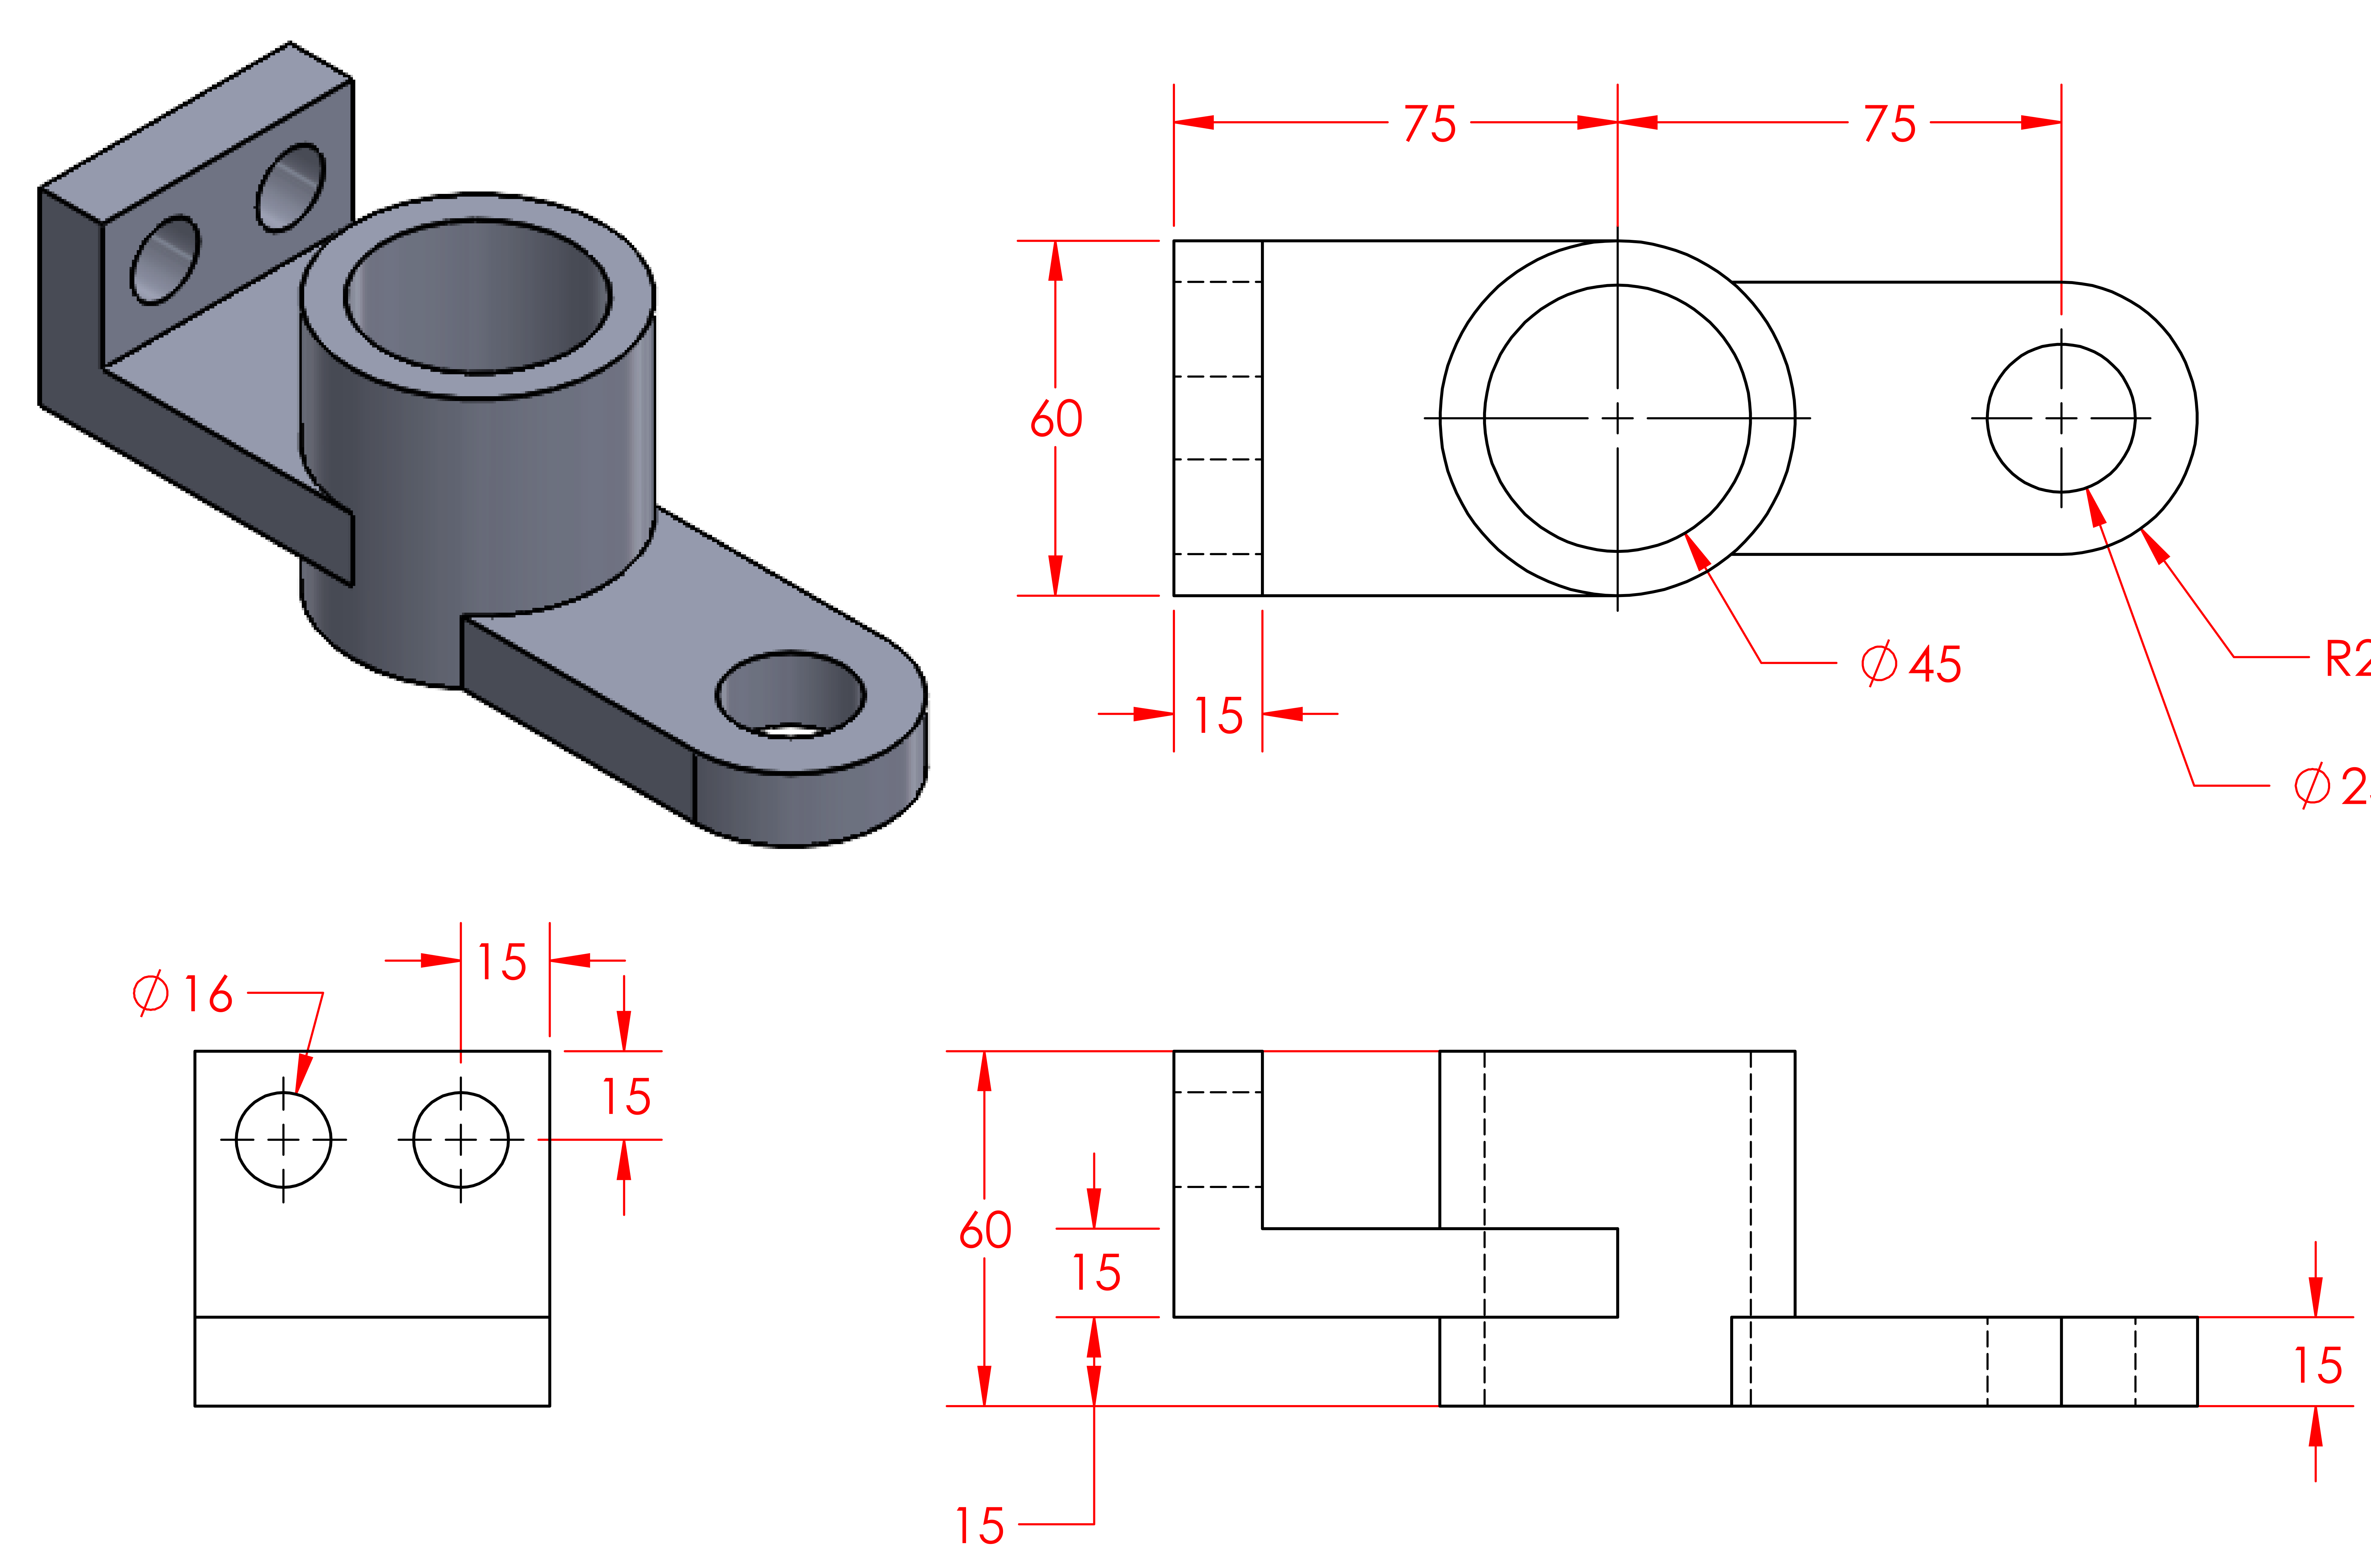
\includegraphics[width=.75\linewidth]{images/8.png}  
  \caption{3D Body}
  \label{fig:8}
\end{figure}
\noindent Please create the 3D body seen above in \textit{Figure 8} using SolidWorks.

%problem 9
\textbf{P9}
\begin{figure}[H]
  \centering
  \includegraphics[width=.68\linewidth]{images/9.png}  
  \caption{Die}
  \label{fig:9}
\end{figure}
\noindent Please create the 3D body seen above in \textit{Figure 9} using SolidWorks.

%problem 10
\textbf{P10}
\begin{figure}[H]
  \centering
  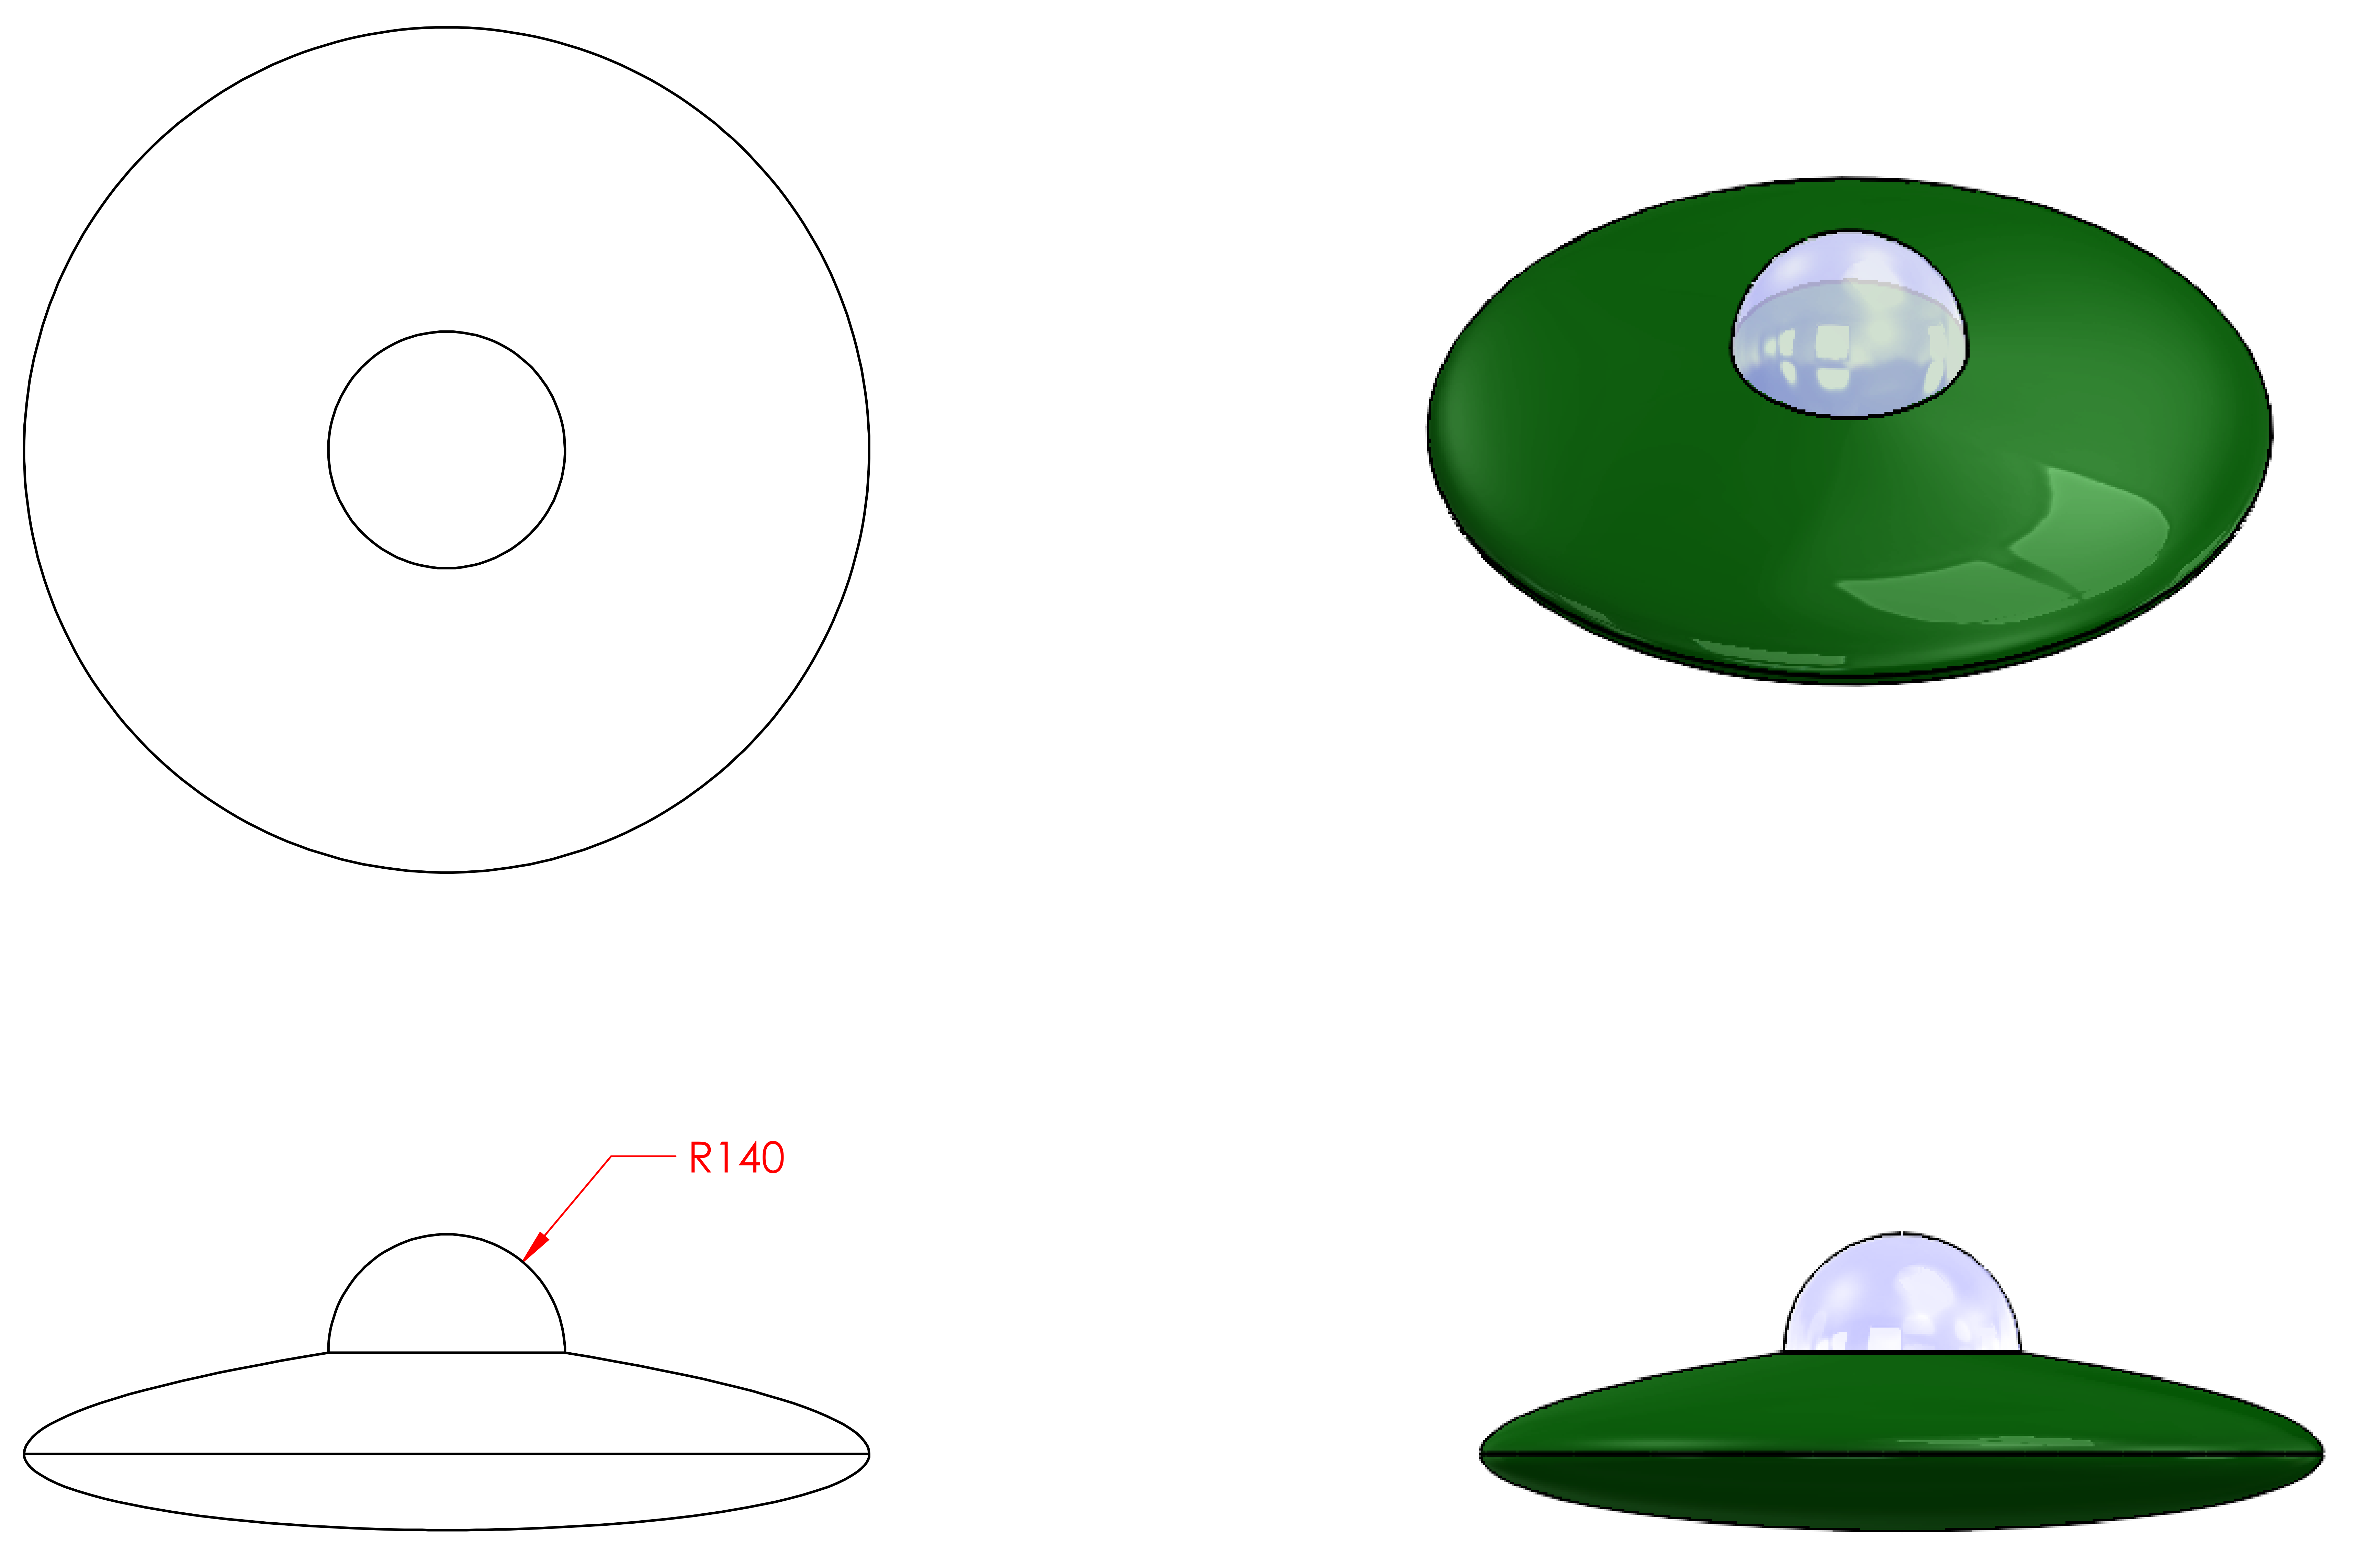
\includegraphics[width=.75\linewidth]{images/10.png}  
  \caption{UFO}
  \label{fig:10}
\end{figure}
\noindent Please create the 3D body seen above in \textit{Figure 10} using SolidWorks.

\end{document}
